\PassOptionsToPackage{usenames,dvipsnames}{xcolor}

% \documentclass[acmtog,anonymous,review]{acmart}
% \acmSubmissionID{1234}
\documentclass[acmtog]{acmart}

\usepackage{booktabs} % For formal tables
\usepackage{xcolor}
% \definecolor{steelblue}{rgb}{0.27, 0.51, 0.71}
\newcommand{\PJ}[1]{\textcolor{CarnationPink}{\bfseries{PJ: {#1}}}}
\usepackage{amsmath, nccmath}
% \usepackage{amssymb} % symbol already defined
% \usepackage{newtxmath}
% \usepackage{preamble-math}

\usepackage[T1]{fontenc}
% \usepackage{fixltx2e}

% TOG prefers author-name bib system with square brackets
\citestyle{acmauthoryear}
%\setcitestyle{nosort,square} % nosort to allow for manual chronological ordering



\usepackage[ruled]{algorithm2e} % For algorithms
\renewcommand{\algorithmcfname}{ALGORITHM}
\SetAlFnt{\small}
\SetAlCapFnt{\small}
\SetAlCapNameFnt{\small}
\SetAlCapHSkip{0pt}

% Metadata Information
\acmJournal{TOG}
%\acmVolume{38}
%\acmNumber{4}
%\acmArticle{39}
%\acmYear{2019}
%\acmMonth{7}

% Copyright
%\setcopyright{acmcopyright}
%\setcopyright{acmlicensed}
%\setcopyright{rightsretained}
%\setcopyright{usgov}
%\setcopyright{usgovmixed}
%\setcopyright{cagov}
%\setcopyright{cagovmixed}

% DOI
%\acmDOI{0000001.0000001_2}

% Paper history
%\received{February 2007}
%\received{March 2009}
%\received[final version]{June 2009}
%\received[accepted]{July 2009}



% Document starts
\begin{document}

% Title portion
\title{Single-view TSDF Mesh Noise Reduction under Virtual Light using Differentiable Rendering}

% DO NOT ENTER AUTHOR INFORMATION FOR ANONYMOUS TECHNICAL PAPER SUBMISSIONS TO SIGGRAPH 2019!
\author{PilJoong Jeong}
\orcid{0000-0001-7579-2047}
\affiliation{
 \institution{Gwangju Institute of Science and Technology}
 \streetaddress{123 Cheomdangwagi-ro}
 \city{Buk-gu}
 \state{Gwangju}
 \postcode{61005}
 \country{Republic of Korea}}
\email{piljoong.jeong@gm.gist.ac.kr}

%\renewcommand\shortauthors{Jeong, P. et al}

\begin{teaserfigure}
    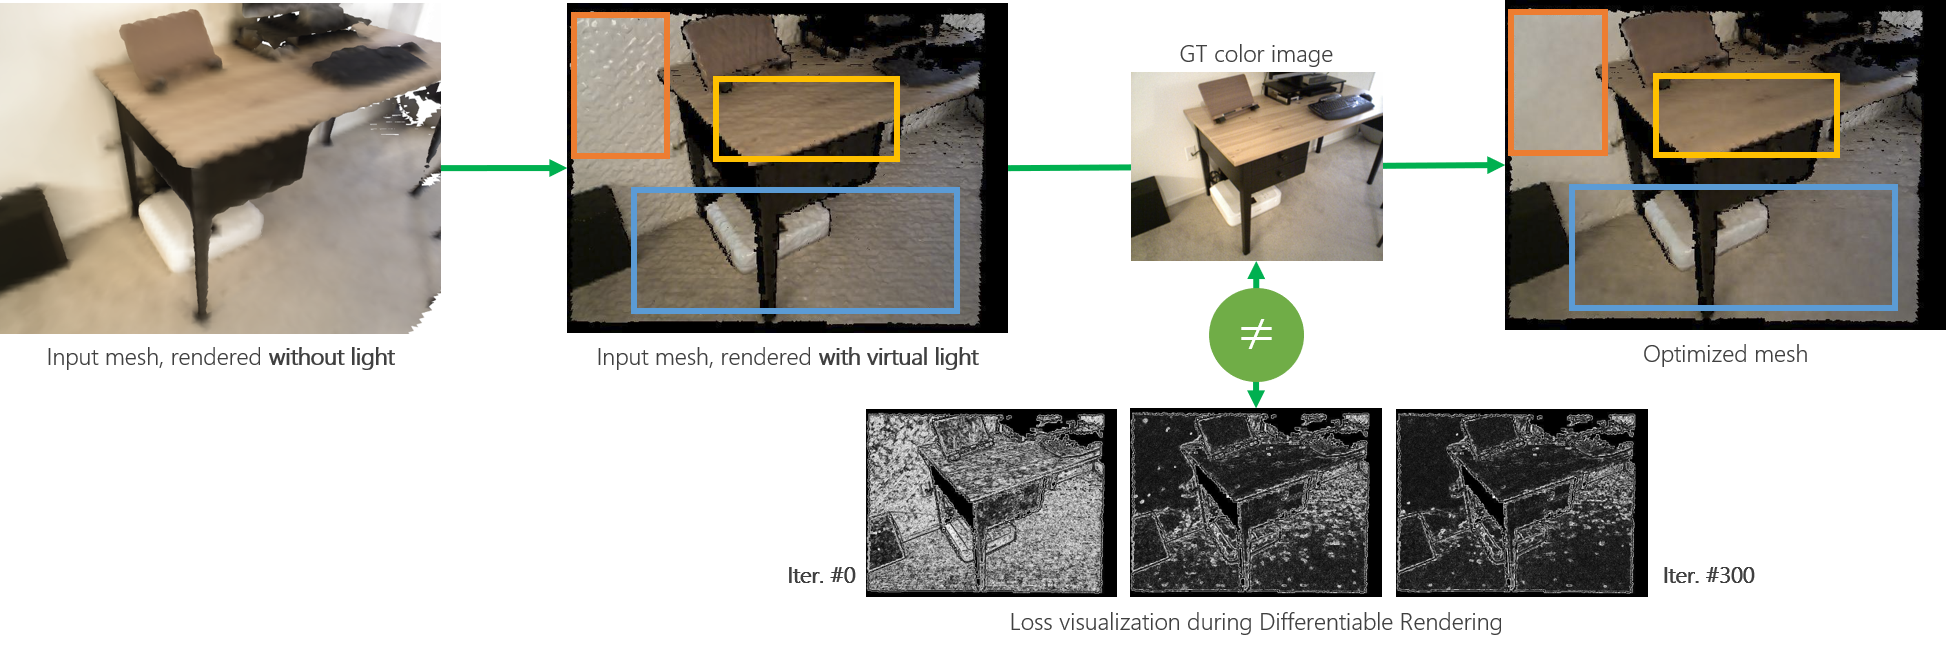
\includegraphics[width=\textwidth]{figures/0_teaser_overview_rev3.png}
    \caption{Overview of our method. (From top left) We saturate noisy vertices by rendering input TSDF mesh with virtually placed light source. We extract common-shared geometric clue between rendered input mesh and target color image. Differentiable renderer iteratively minimizes loss, which is the difference between clues from rendered input mesh and target Ground Truth color image. Orange, Yellow, and Blue inset shows difference between input mesh and optimized mesh. Our method successfully reduces noise in mesh vertices. Furthermore, our provided video shows input mesh that is being optimized (right-side of the video) as iteration continues, as well as the visualization of loss (left-side of the video) that is being minimized: \url{https://drive.google.com/file/d/10F_I89m5O-RWOIxocYoxG2QOkJc7YWlF/view?usp=sharing} \PJ{TODO. change url to personal drive.}}
    \label{fig:teaser}
\end{teaserfigure}

\begin{abstract}
Thanks to consistent evolution of SLAM (Simultaneous Localization and Mapping) and its related technologies, we can reconstruct geometric properties of where we are currently observing in real-time. Due to the limitation of current depth sensing hardware, however, we are generally able to obtain geometric features corrupted by noise. Color image is perceived as geometrically noise-free in terms of human vision-perception system, but to our best knowledge, encoding the information from Ground Truth for differentiable rendering under single view constraint is not discussed yet. In this report, we propose a bridge between the geometric information generated from color image and rendered mesh, so that differentiable renderer can optimize input i.e., noisy vertex position without any depth supervision. The key insight is that we can highlight noisy vertices by rendering mesh with virtually placed light sources. We compare our result with one of the state-of-the-art differentiable rendering method[1], and show our method outperforms previous method which requires prior depth information (silhouette image).
\end{abstract}

%
% The code below should be generated by the tool at
% http://dl.acm.org/ccs.cfm
% Please copy and paste the code instead of the example below.
%
\begin{CCSXML}
<ccs2012>
    <concept>
        <concept_id>10010147.10010371.10010396</concept_id>
        <concept_desc>Computing methodologies~Shape modeling</concept_desc>
        <concept_significance>500</concept_significance>
        </concept>
    <concept>
        <concept_id>10010147.10010371.10010387.10010392</concept_id>
        <concept_desc>Computing methodologies~Mixed / augmented reality</concept_desc>
        <concept_significance>500</concept_significance>
        </concept>
    </ccs2012>
\end{CCSXML}
\ccsdesc[500]{Computing methodologies~Shape modeling}
\ccsdesc[500]{Computing methodologies~Mixed / augmented reality}
%
% End generated code
%


\keywords{Differentiable rendering, Mesh denoising}

\maketitle

\section{Introduction}

To satisfy increasing demand of 
Augmented Reality (AR) technology, we required to obtain geometric information of observed real scene as precise as possible. 
As precision of geometric detail is increased, we can augment virtual objects with more consistency from computer graphics (Photorealistic Rendering) perspective, and we are able to estimate camera poses from perfect correspondences from computer vision (Simultaneous Localization and Mapping; SLAM) perspective.

Capturing detailed geometry is still remain as technical challenge due to hardware/computational limitation of SLAM. 
It is obvious that consumer-level depth sensing technology still has noisy observation. 
We can cope this by divide a real scene with less detailed (coarse) voxels to smooting out noisy depth measurements when generating TSDF mesh. 
In this way, however, it fails to retain geometric detail even in the case of reconstructing perceptually simple geometry (e.g., edge between planes).
To preserve geometric detail, we still need to divide voxels as fine as possible where is geometrically complex. 
This directly affects to rendering performance, as rendering requires primitive traversal in order to appropriately propagates lighting information for every single frame. 
Due to those limitations, we are compromised to use TSDF meshes from acceptably coarse voxels, which have geometric incorrectness including noise. 
Nevertheless, there is strong demand to perfect geometry captured from SLAM sequences. 

Recent advances of Differentiable Rendering make it possible to optimize current input parameters by observing a set of given Ground Truth images. 
This seems promising to SLAM, as they naturally capture Ground Truth color images whereas generating input TSDF mesh corrupted by noisy measurements. 
However, it is unclear that how to interpret (perceptually encoded) geometric clues within color images, reflect those information into actual geometry to minimize its imperfection. 
Moreover, there is some limitations hinder directly applying previous differentiable rendering techniques into SLAM dataset. 
We explained such difficulties in (Fig. \ref{fig:difference_simple_mesh_and_tsdf_mesh}).

Our main contribution is bridging the gap between perceptional noise-free geometric features from input color image and noisy geometric feature in input mesh. 
To exploit this, we interpreted input color image as a result of perfect renderer with perfect geometry. 
Under certain assumptions, we argued that radiance is consistent if a point and its neighbors are lie on a same plane.
Generally, it is not true for virtually rendered image with input mesh, as the mesh is composed with noisy vertices.
Therefore, we optimized input mesh to have radiance consistency i.e., noise-free geometry which is input color image have.

% \PJ{TODO: move this into method; this is not our main contribution, rather it is close to implementation detail.}
% To exploit this, we borrow a novel concept of image denoising using flashlight. Images taken with flashlight can hold additional features which are hard to detect from general geometric feature (e.g., depth, normal etc). 
% For example, in \cite{eisemann2004flash} \cite{petschnigg2004digital} flashy photography is used to enhance images taken from scene which has insufficient lighting condition. 
% \cite{moon2013robust} is pioneering work that adopt image enhancement using flashlight on photorealistic rendering domain, by casting virtual flashlights to capture a scene’s reflective / refractive features, which are not stored in traditional G-buffers. 
% Based on these approaches, we saturate noisy vertices by casting virtual light, which are never detected when rendered with mesh’s albedo only. 
% Please refer the leftmost image (rendered without light) and its connected image (rendered with virtual light) in \ref{fig:teaser} for details. 
We demonstrate our results, compare with result from previous method, and show that our method outperforms previous result.
\section{Previous Works}

\paragraph{TSDF Mesh Noise Reduction in SLAM}
Starting from pioneering work [5], 
estimating true depth from noisy measurements 
has been one of the major challenges in SLAM. 
Basically, [5] first introduced the definition of ‘fusion’, 
which is accumulating noisy world positions into a voxel. 
This acts as similar with spatial running average filter, 
therefore it is known that accumulating frames 
that captures same region can reduce noise incrementally. 
However, this takes a lot of time to converge depth values 
to a true mean, which interferes practical AR application experience. 
Therefore, various depth noise reduction techniques are applied to SLAM systems, 
including simple bilateral filter [6],  merging depth information of neighboring frames either offline [7][8], or online [9][10]. 
All mentioned previous works require multiple depth frames 
in order to generate reliable mesh which takes a long time, 
and they did not consider color images, which holds perceptive geometric information. 
Our method, in contrast, is able to infer geometric clue in color image, 
thus able to de-noise input mesh without multiple frames.

\paragraph{Differentiable Rendering}
Differentiable rendering is the technique that 
optimizing input parameters by observing a set of target images 
via iteratively render a scene with current state of input parameters (i.e., forward pass), 
as well as propagate gradients along with computation graph (i.e., backward pass) built at forward pass. 
Due to the fact that it does not require any prior knowledge (e.g., pre-trained model trained from external dataset) 
other than target images, this seems an off-the-shelf optimizer for SLAM 
since we naturally capture target image during scanning process, 
whereas fused mesh is contaminated with noise due to its nature limitations. 
However, there are ambiguities that have to be considered 
in order to adapt differentiable rendering to optimize SLAM problems. 
Figure 2. describes the different setup between simple mesh optimization 
and indoor TSDF mesh optimization. 
Our method bypasses those ambiguities via inferring geometric clue 
without necessity of silhouette information, as well as multiple target observations.
\begin{figure}
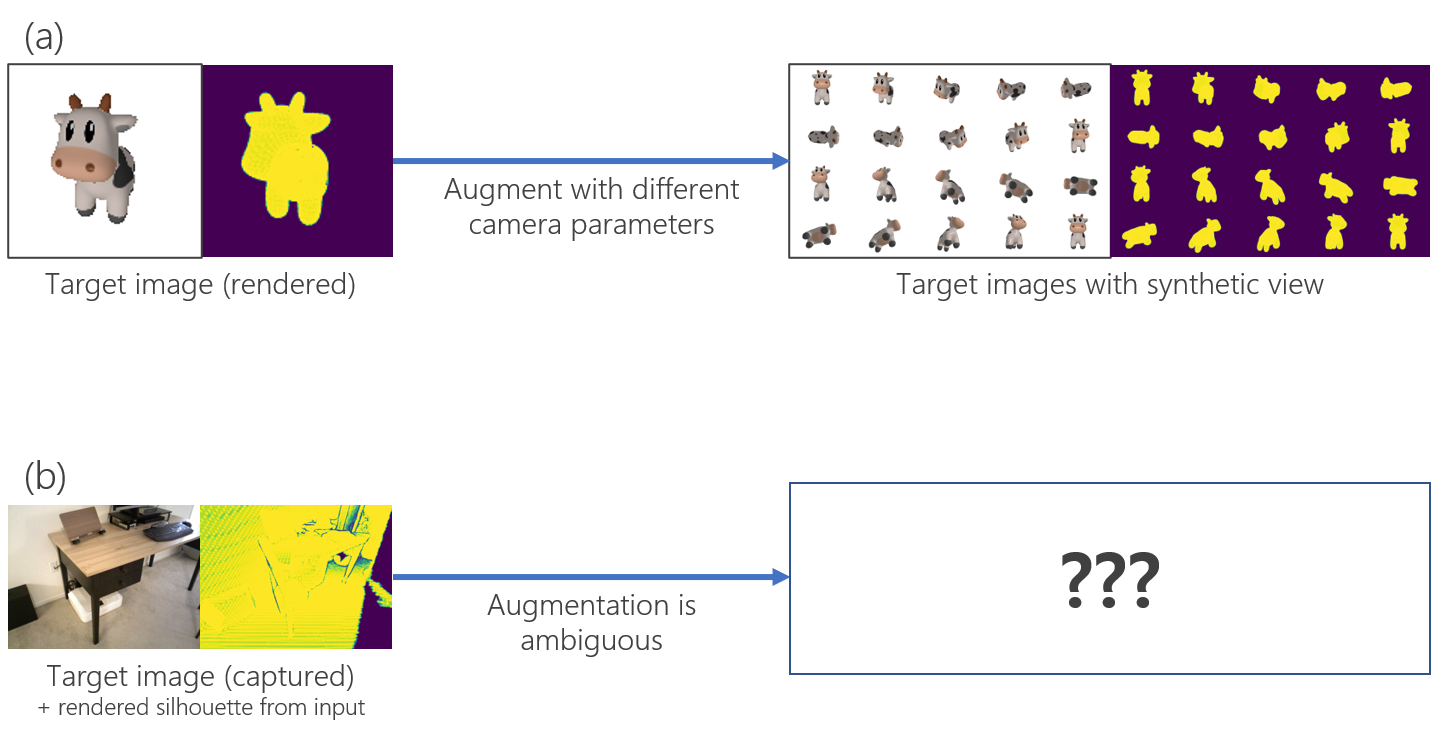
\includegraphics[width=\columnwidth]{figures/2_prev_difference_simple_mesh_and_tsdf_mesh.png}
\caption{Different setup between optimizing simple mesh and TSDF mesh from SLAM. Previous works aimed to optimize input geometry to set of target images captured with different camera view either synthetically[11][12][13][14] or by taking calibrated real photographs[14]. However, in the case of TSDF mesh from SLAM it is ambiguous since (1) input is not separated with its backgrounds, hence silhouette image is hard to generate (2) we cannot generate synthetic target views (3) it is hard to sample real images from SLAM sequences which captures a region that input mesh represents, since the labeled camera pose paired with target image is estimated value. It is well-known that camera poses from SLAM is inaccurate. (a) It is straightforward to generate synthetic target images if the target image can be rendered. (b) Unlike (a), it is much hard to augment target images in order to optimize indoor TSDF mesh.}
\label{fig:two}
\end{figure}
\section{Methods}

We propose an optimization procedure that incrementally minimizes mesh vertex noises using differentiable rendering. 
Suppose we have vertices $V=\{V_i\in\mathbb{R}^3\}=\{V_0...V_n\}$ within input mesh $\mathcal{M}$ which is fused from input color $\mathcal{C}$ and depth $\mathcal{D}$ with intrinsic $K$ such that $\mathcal{M}=K^{-1}\left(\mathcal{C}\oplus \mathcal{D}\right)$. 
Here, $\oplus$ denotes image registration operator.
We pre-computed $\mathcal{M}$ from popular off-line SLAM framework \cite{zhou2018open3d} with voxel size 2cm.
We define deformed vertices $V_d$, which has same shape as $V$ initialized with zero values i.e., $V_d=\{\mathbf{0}_0,...,\mathbf{0}_n\}$. 
For every iteration, $V_d$ is optimized so that resulting vertices $V_o=V+V_d$ approximate noise-free geometry which looks perceptually similar with $\mathcal{C}$. 
\PJ{Emphasize minimizing difference between GT color and rendered color.}
The main problem is how to find common geometric representations between $\mathcal{C}$ and $C$ to figure out which region is to be optimized (i.e., noisy).

\paragraph{Assumptions}
Our goal is to minimize vertex noise of TSDF mesh $\mathcal{M}$ fused from a single pair of indoor RGB-D images $\mathcal{C}\oplus \mathcal{D}$. Given this scenario, we assume that we known camera intrinsic $K$ and extrinsic $T=I\in\mathbb{R}^{4*4}$. 
We will also consider the captured real scene is Lambertian, as all SLAM datasets are generated under Lambertian-dominant assumption to guarantee accurate camera pose estimate, unless additional consideration of non-Lambertian scene is introduced. \PJ{TODO: refer [Whelan, 2018]}
We additionally constrain that there are no strong texture changes under geometrically close, flat surfaces. 

\subsection{Interpreting Perceptually Noise-free Geometry from Color Image}
\PJ{Too verbose! TODO: add proof}
In this section, we formally describe our intuition that enables input color image treated as noise-free geometric clue.

Let us consider $\mathcal{C}$ as a result from perfect renderer which is capable of tracing full light transport without any noise and outlier, given unknown lighting conditions and noise-free geometry. 
Based on Light Transport Equation(LTE) representation with respect to path integral form \cite{veach1998robust}, we represent $\mathcal{C}$ as a set of solution of LTE for each pixel:

\begin{align}
    \mathcal{C} & = \bigcup_i^W \bigcup_j^H L_{i,j}\left(K^{-1}\cdot x\rightarrow p_0\right) \nonumber \\
    & = \bigcup_i^W \bigcup_j^H L_{i,j}\left(p_1'\rightarrow p_0\right),
\end{align}
where $L_{i,j}$ is total radiance at a pixel, and $p_1'=K^{-1}\cdot x$ is hitpoint of $L_{i,j}$.

To intuitively exploit relationship between $\mathcal{C}$ and noise-free hitpoint $x_{i,j}$, we expand radiance sum over path:
\begin{align}
    L_{i,j}\left(p_1'\rightarrow p_0\right)& = [\mathit{P\left(\bar{\mathrm{p}}_1\right)}+\mathit{P\left(\bar{\mathrm{p}}_2\right)}]+[\sum_{n=3}^\infty \mathit{P}\left(\bar{\mathrm{p}}_n\right)], 
    \label{LTE_path_integral}
\end{align}

where $\bar{\mathrm{p}}_n=\mathrm{p}_0\mathrm{p}_1...\mathrm{p}_n$ is path segment with $n+1$ vertices. We examine emitted radiance i.e., Albedo and direct lighting term in (Eqn. \ref{LTE_path_integral}):

\begin{align}
    \mathit{P\left(\bar{\mathrm{p}}_1\right)}+\mathit{P\left(\bar{\mathrm{p}}_2\right)}=\int_A & f\left(p_2\rightarrow p_1\rightarrow p_0\right)\cdot L_{e (i,j)}\left(p_2\rightarrow p_1\right)\cdot \nonumber \\
    & V\left(p_1 \leftrightarrow p_2\right) \cdot dA\left(p_2\right)
\end{align}


% Our key observation is strong radiance change within color images $\mathcal{C}$ and $C$, is only occurred from strong geometric displacements around a corresponding pixel. 
% This is possible since we made two assumptions: Lambertian-dominant scene, and no strong texture changes under flat surface. 
% Consider $\mathcal{C}$ is generated from perfect renderer 
% which are capable of tracing full light transport, under perfect geometries. 
% Although we cannot know which lighting conditions are used to render $\mathcal{C}$, 
% however, at least we know the lighting is somehow applied to 
% perfect geometries since $\mathcal{C}$ is rendered, as well as we are able to perceive geometric information by just observing $\mathcal{C}$. 
% Using the fact that $\mathcal{C}$ is a discretization of continuous radiance function, 
% we can intuitively notice that changing lighting condition 
% never affects to local radiance change (unless the light is very close to the surface).
% From this intuition, we can render $\mathcal{M}$ over virtually placed light source(s). 
% If $\mathcal{M}$ is noise-free enough, there would be no highlighted pixel in its rendering $C$. 
% However, due to the fact that $C$ is rendered with $\mathcal{C}$ from noisy measurement $\mathcal{D}$, 
% there exist a set of saturated pixel, which are actually not saturated within $\mathcal{C}$. 
% Based on this observation, we decided to minimize gap between saturated pixels in $C$ and unsaturated i.e., noise-free pixels in $\mathcal{C}$. 
% In order to do this, it is required to detect noise-free pixels in $\mathcal{C}$, as well as noisy pixels in $C$, 
% and set the difference as loss function so that our differentiable renderer properly minimizes gap.

\subsection{Detecting Geometric Information given Color Image and Its Rendering}
We simply detect noise-free surfaces within $\mathcal{C}$ by applying Scharr gradient kernel. 
Under the assumption that the scene is Lambertian-dominant and there is no sudden strong texture changes around the same surface, 
we found that this is enough to capture which region is smooth in terms of radiance (i.e., geometrically noise-free). 
In order to ensure robustness on strong texture changes 
one may combine with gradient from $\mathcal{D}$, but for this report we only experimented with gradients from $\mathcal{C}$. Specifically, Scharr kernel for each axis over an image is defined as
\begin{equation}
    \label{eqn:01}
    G_x=\begin{pmatrix}
        -3 & 0 & 3\\
        -10 & 0 & 10\\
        -3 & 0 & 3
    \end{pmatrix}, 
    G_y=\begin{pmatrix}
        -3 & -10 & -3\\
        0 & 0 & 0\\
        3 & 10 & 3
    \end{pmatrix}
\end{equation}
, and our detected geometric changes over Ground Truth color image $\widetilde{G}_\mathcal{C}$ is a Scharr gradient of $I_\mathcal{C}$ i.e., the intensity image from $\mathcal{C}$. 
Since resulting gradient on some pixels have negative value of identical magnitude to positive values of neighboring pixel, we take its absolute value
\begin{equation}
    \label{eqn:02}
    \widetilde{G}_\mathcal{C}=\frac{1}{2}\left(|G_x\left(I_\mathcal{C}\right)|+|G_y\left(I_\mathcal{C}\right)|\right)
\end{equation}
In order to detect noisy vertices over TSDF mesh, we propose Lightweight map to determine which vertex has stronger noise compare to $\widetilde{G}_\mathcal{C}$. 
Lightweight map $I\textsubscript{lw}$ is an image taken from identical camera setup to $\mathcal{C}$, but holds how much a pixel corresponds to a hitpoint is affected by virtual light at a shading stage.
$I\textsubscript{lw}$ is defined as
\begin{equation}
    I\textsubscript{lw}=\{I\textsubscript{lw,i}\in\mathbb{R}\textsuperscript{\textit{W}*\textit{H}}\}, I\textsubscript{lw,i}=\frac{\left(x_i-p_0\right)\cdot n_i}{d\left(x_i,p_0\right)+\epsilon}, 
\end{equation}
where $x_i$, $n_i$ is world position and normal of hitpoint with pixel index \textit{i}, respectively. 
$p_0$ is position of virtual light, and $d\left(x_i, p_0\right)$ is Euclidean distance between hitpoint and light position.
We obtain changing amount of each lightweight value $\widetilde{G}\textsubscript{lw}$ by applying Scharr kernel over $\textit{I}\textsubscript{lw}$, similar with $\widetilde{G}_\mathcal{C}$.
\begin{equation}
    \widetilde{G}_\textsubscript{lw}=\frac{1}{2}\left(|G_x\left(I\textsubscript{lw}\right)|+|G_y\left(I\textsubscript{lw}\right)|\right)
\end{equation}
We found that using geometric normal to calculate lightweight map saturate pixels around noisy vertices rather than shading normal, 
as shading normal smooths normal of each hit-point using neighboring vertex normal and its barycentric coordinates. 
In detail, pixels within same face have similar lightweight values 
since they are both geometrically close to each other, and they share same normal. 
Pixels that are geometrically close, but within different faces 
are highly likely to have similar values if two faces have near identical normal values. 
This is the case when two faces are considered as ‘flat’ to each other, 
meaning that shared vertices have no noise. 
As the vertex have bigger noise, the gap or normal between sharing two faces also gets bigger. 
This brings pixels in $G\textsubscript{lw}$ have large value where there is significant normal difference, meaning that the region has noisy vertex. 
Note that larger $G\textsubscript{lw}$ at a pixel means that the pixel has higher noise, therefore differentiable renderer can optimize the region more aggressively. 
This is illustrated in Figure 3.
We observed that the intensity image of rendered scene with virtual light $I_C$ serves similar role with $I\textsubscript{lw}$ as they properly reflect strong gradients around deviating normal.
Therefore, we note that for all results we used $I_C$ instead of $I\textsubscript{lw}$.
\begin{figure*}
    \centering
    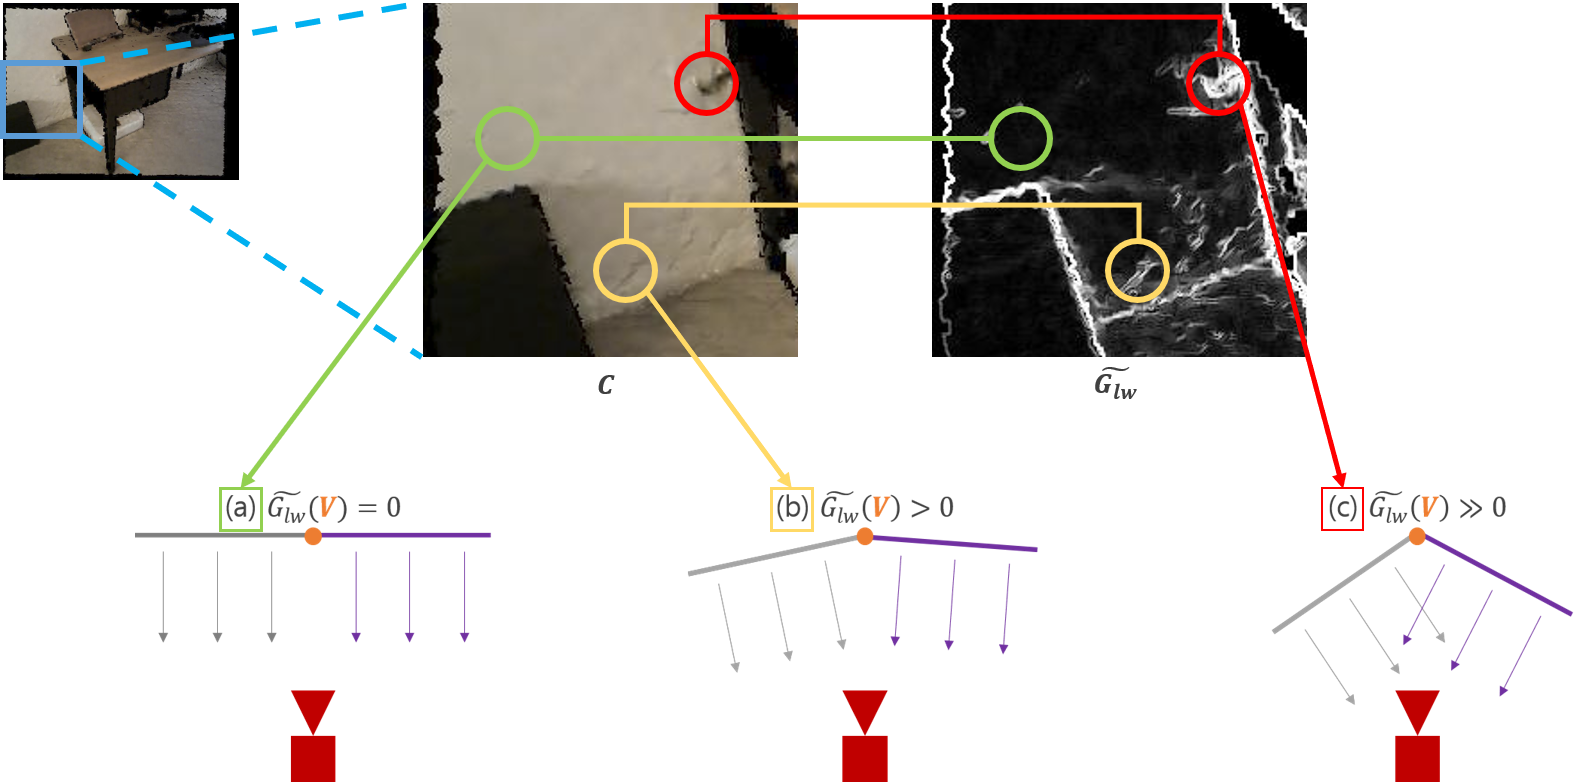
\includegraphics[width=\textwidth]{figures/3_method_relationship_gradient_lightweight_and_noise_full_tone_changed.png}
    \caption{Relationship between $G\textsubscript{lw}$ and actual noise of vertex $\textcolor{Orange}{V}$. We manually selected three pixels, where each have different magnitude of $G\textsubscript{lw}$. We also illustrated 1D example of the relationship. \textbf{\textcolor
    {Gray}{Gray}} and \textbf{\textcolor{Purple}{Purple}} lines and arrows indicate each face and its geometric normal. \textbf{\textcolor{LimeGreen}{(a)}} $\textcolor{Orange}{V}$ is considered as noise-free since $G\textsubscript{lw}$ is evaluated as zero, meaning adjacent faces have identical normal value. \textbf{\textcolor{Dandelion}{(b)}} $G\textsubscript{lw}$ is increased as two faces have inconsistent normal. \textbf{\textcolor{Red}{(c)}} as $G\textsubscript{lw}$ gets bigger, $\textcolor{Orange}{V}$ is considered as highly-noisy vertex. From these examples, we can say that $G\textsubscript{lw}$ precisely indicates where noisy pixels exist.}
    \label{fig:relationship_gradient_lightweight_and_noise}
\end{figure*}

\subsection{Optimization using Differentiable Rendering}
We define lightweight loss to minimize the difference between noise-free geometric information $\widetilde{G}_\mathcal{C}$ and noise-detected rendered image $\widetilde{G}_C$. We found that there is gradient value range inconsistency between $\widetilde{G}_\mathcal{C}$ and $\widetilde{G}_C$, as they are derived from different type of image i.e., color and geometry, respectively. We applied hyperbolic tangent kernel to each gradient image to ensure that both images have normalized value range, and we observed that this helped optimizer to find optimal without failure. Finally, we replace our target GT image from $\mathcal{C}$ to $\mathcal{C}\oplus\mathcal{D}$, as $\mathcal{M}$ follows holes where pixels in $\mathcal{D}$ have zero value. Our final geometric gradients are:
\begin{equation}
    G_\mathcal{C}=\tanh\left(\widetilde{G}_{\mathcal{C}\oplus\mathcal{D}}\right),
    G_{lw}=\tanh\left(\widetilde{G}_{lw}\right), 
\end{equation}
where $\tanh\left(x\right)=\frac{e^x-e^{-x}}{e^x+e^{-x}}$. Our optimizer minimizes lightweight loss representing geometric difference, while penalizing vertices not to evolve too far from its initial position:
\begin{gather}
    \mathcal{L}=w_{lw}\cdot L_{lw}+w_{pos}\cdot L_{pos}, \\
    L_{lw}=\left|\left|G_\mathcal{C}-G_C\right|\right|^2_2, \\
    L_{pos}=\left|\left|V-\left(V_o\right)\right|\right|^2_2=\left|\left|V_d\right|\right|^2_2
\end{gather}
For all results, we used $w_{lw}=0.01$ and $w_{pos}=1.0$. Fig. 4 visualizes optimization procedure.
\begin{figure}
    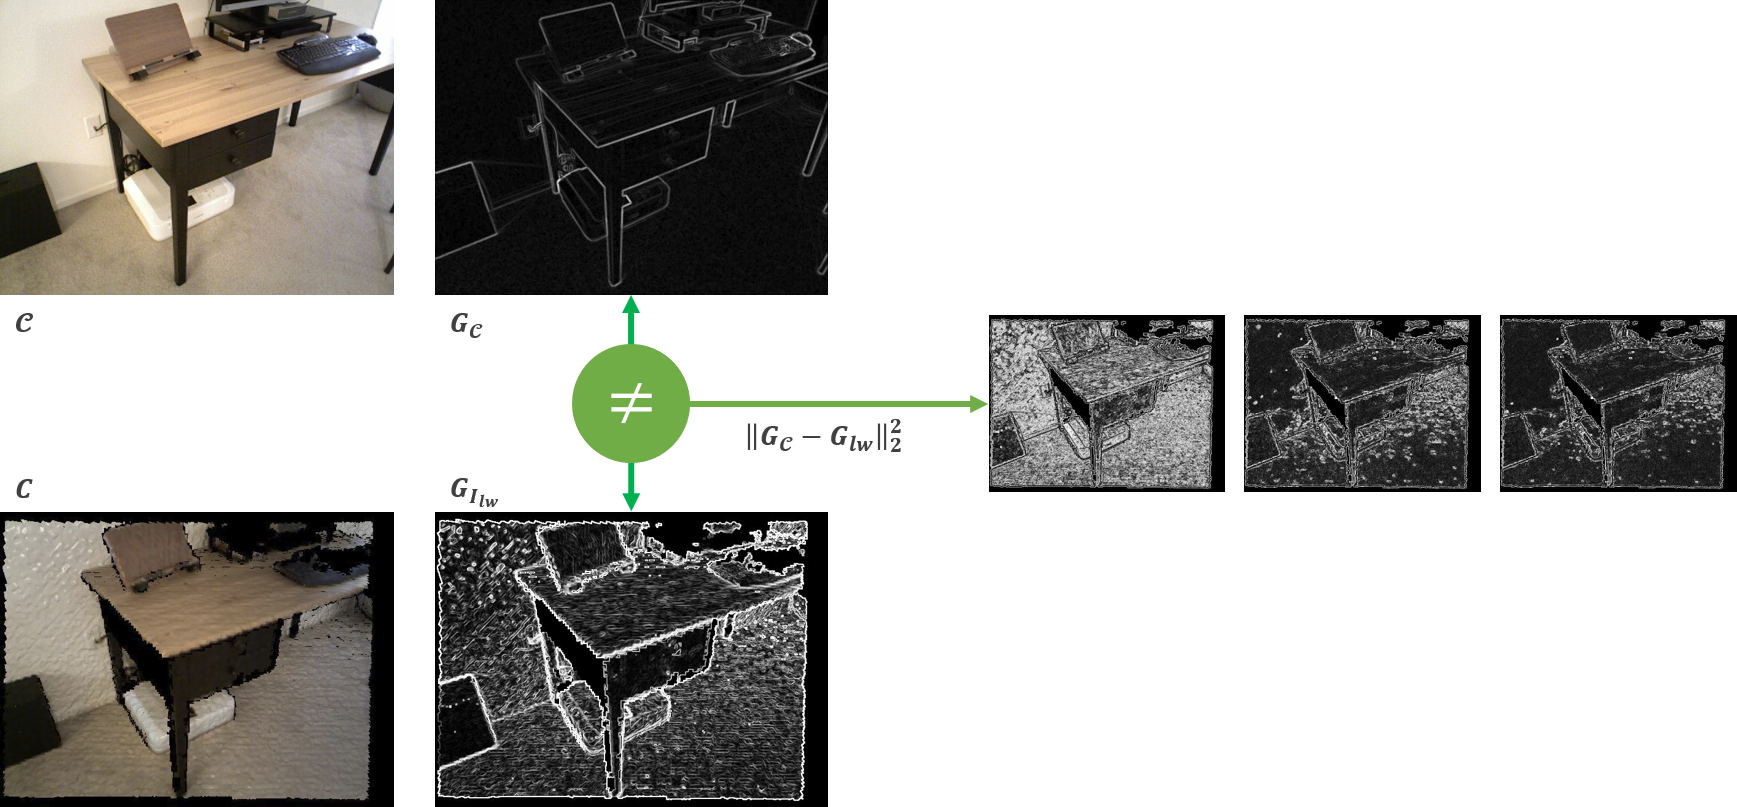
\includegraphics[width=\columnwidth]{figures/3_method_optimization.png}
    \caption{Optimization procedure of our differentiable rendering. From generated target noise-free geometric clue $G_\mathcal{C}$ and input noisy geometric clue $G_{lw}$, we minimize $L_2$ distance between two clues. Note that we additionally penalize aggressive vertex evolve, however it is skipped in the figure.}
    \label{fig:optimization}
\end{figure}
\section{Results}
We have implemented our method on top of general differentiable renderer\cite{ravi2020accelerating}. 
For all tests, we used Intel Xeon E5-2687W CPU machine with 3.0GHz, and GeForce RTX 2080 TI for CUDA-optimized differentiable renderer. 
We optimized our mesh with Stochastic Gradient Descent method with learning rate = 1.0, and momentum = 0.9. 
For $\mathcal{M}$, we pre-computed from popular off-line SLAM framework \cite{zhou2018open3d} with voxel size 2cm.
We placed one virtual light source at the camera center for all experiments, although this method is up to a number of lights and its positions.


\subsection{Validation of Proposed Method}


\begin{figure}
    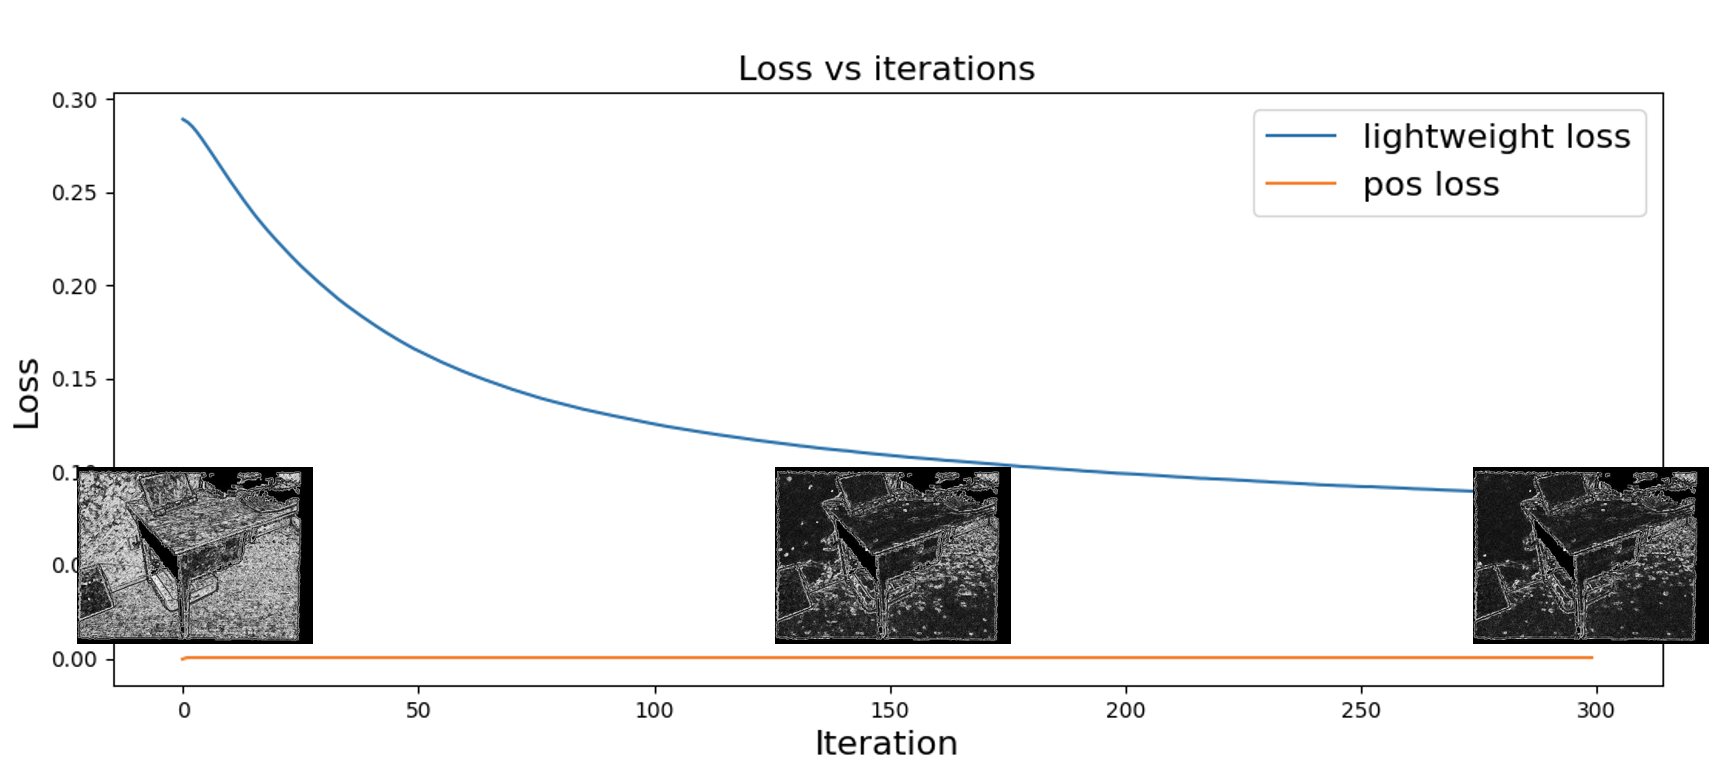
\includegraphics[width=\columnwidth]{figures/4_result_loss_plot_with_images.png}
    \caption{Loss plot with loss images at specific iterations (here, 0, 150, and 300 is used). Our lightweight loss successfully minimizes vertex noise by observing target noise-free geometric information $G_\mathcal{C}$. Note that $L_{pos}$ never converges to zero, as they act as constraint to vertices not to evolve too far from its original position, thus have non-zero values among all iterations.}
    \label{fig:loss_plot_with_images}
\end{figure}

\begin{figure}
    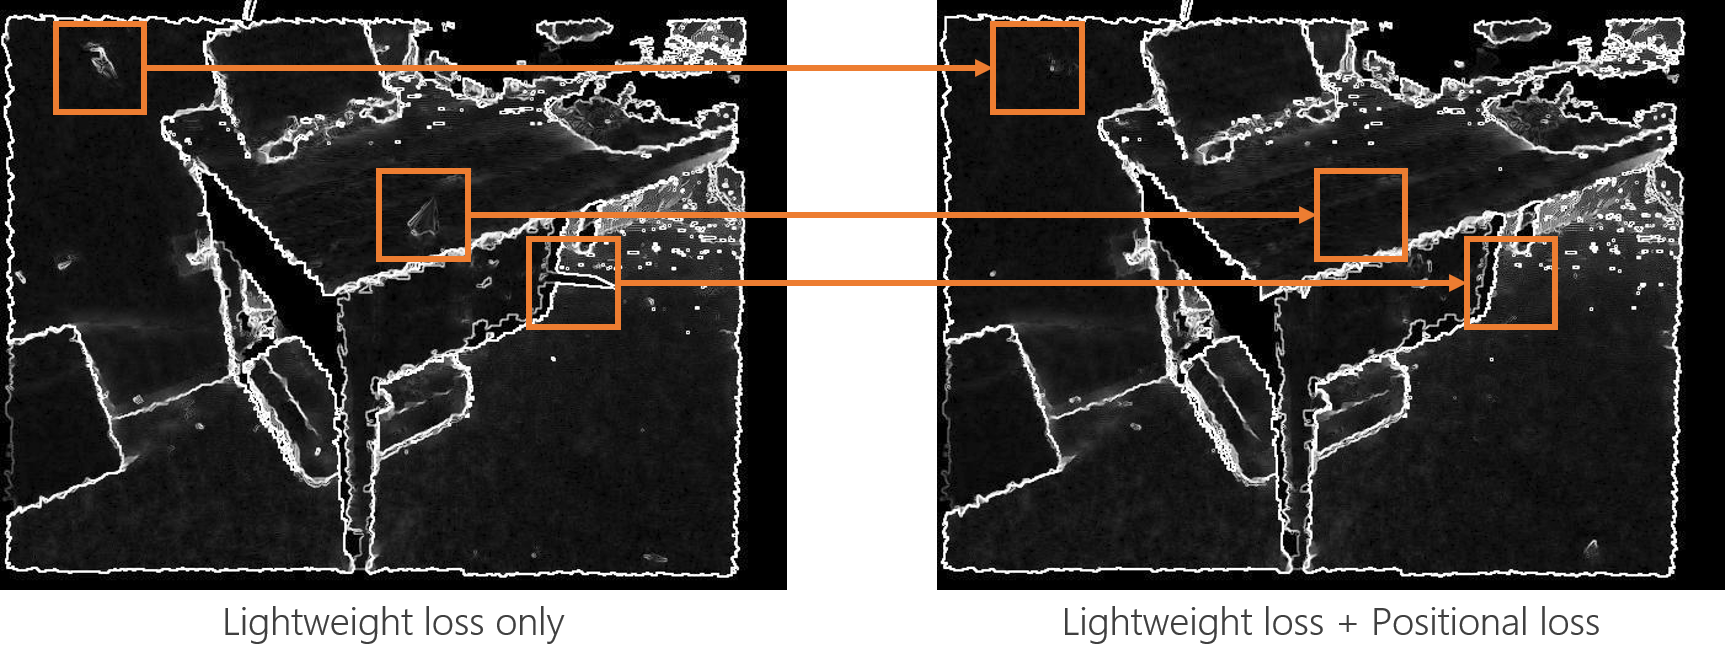
\includegraphics[width=\columnwidth]{figures/4_result_ablation_study_positional_loss.png}
    \caption{Ablation study of positional loss, without loss and with loss, respectively. \textcolor{Orange}{\textbf{Orange}} inset highlights difference of vertex evolving aspect. Note that total loss of both result is converged. (Left) Some vertices are evolved in a wrong direction with respect to its perceived shape (Right) Our result with positional loss successfully maintain its shape, as the loss prevent vertices evolve not too far from its original position.}
    \label{fig:ablation_study_positional_loss}
\end{figure}

\paragraph{Validation of loss}
In (Fig. \ref{fig:loss_plot_with_images}), we plotted our loss graph to ensure that our loss function forms a convex function. 
Our proposed lightweight loss is monotonically decreased as the optimization continues. 
Note that our positional loss is not minimized, as we want positional loss to act similar with regularization term, which prevents evolving vertices getting not to far from its original position. 
Nevertheless, the total loss forms a convex function as the actual contribution of positional loss is small enough than lightweight loss. 
We showed the effect of positional loss in (Fig. \ref{fig:ablation_study_positional_loss}).

\paragraph{Validation with various scenes}


\begin{figure*}
    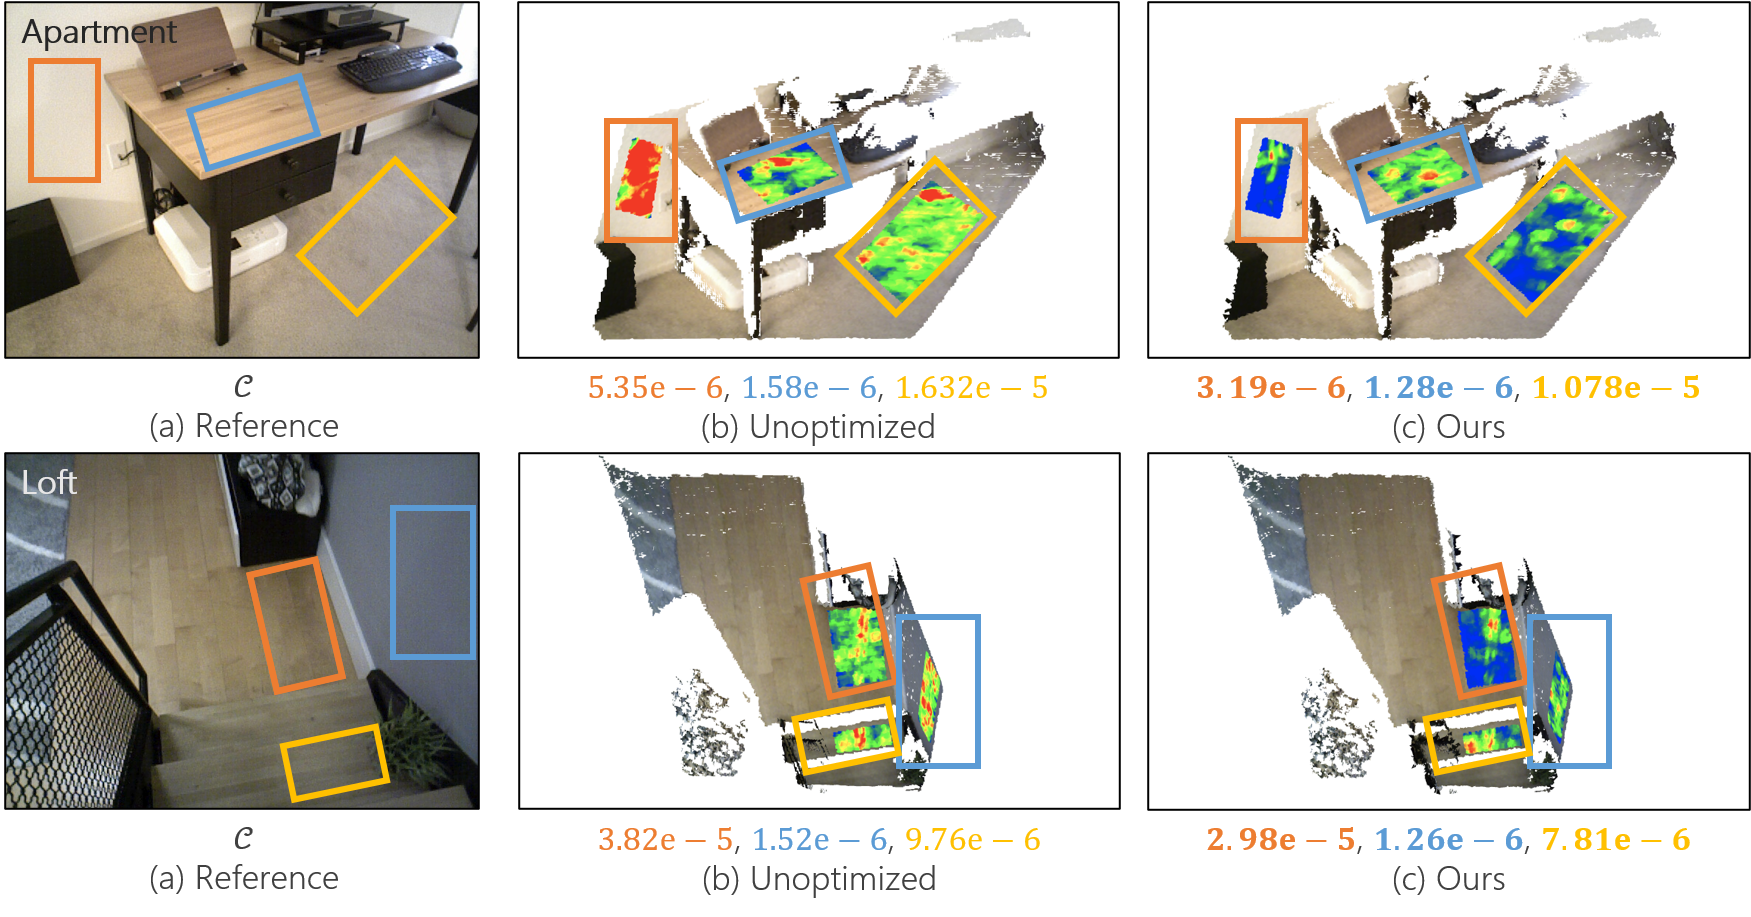
\includegraphics[width=\textwidth]{figures/4_result_plane_fitting_all.png}
    \caption{Plane fitting validation of our result. Given scenes (Left), we selected \textcolor{Orange}{\textbf{Orange}}, \textcolor{NavyBlue}{\textbf{Blue}}, and \textcolor{Dandelion}{\textbf{Yellow}} regions where are considered as "perceptually flat". We compared minimum eigenvalue of hitpoint $\lambda_3$ between insets of input mesh (Middle) and optimized mesh (Right), and visualized heatmap of each result. Heatmap indicates \textcolor{NavyBlue}{blue} if a region is totally flat i.e., $\lambda_3 \approx 0$, and colored \textcolor{Red}{red} vice versa. For each inset, we additionally report maximum value of $\lambda_3$, and marked as boldface where has lesser $\lambda_3$. }
    \label{fig:result_plane_fitting}
\end{figure*}

We validated performance of our proposed method, by evaluating minimum eigenvalue $\lambda_3$ of the region where we are able to perceive as 'flat', given $\mathcal{C}$.
Particularlly, for each selected inset, we cropped input and optimized mesh, and sampled sufficient amount (e.g., 1M) of point cloud. 
$\lambda_3$ is computed for each point cloud, by running Principle Component Analysis to spatial covariance matrix $\Sigma_i=\frac{1}{N}\sum_{\mathrm{n}\in\mathcal{N}}(\mathrm{p_n}-\bar{\mathrm{p}})(\mathrm{p_n}-\bar{\mathrm{p}})^T$, which generates eigenvalues $\lambda_1 \ge \lambda_2 \ge \lambda_3 \ge 0$. 
As $\lambda_3$ goes close to zero, $\Sigma_i \in \mathbb{R}^3$ represents distribution of points projected in a plane.
Intuitively, we can consider optimization is succeed if $\lambda_3$ is decreased compare to input mesh for each points.
To validate this, we plotted heatmap of $\lambda_3$ for each points in (Fig. \ref{fig:result_plane_fitting}).
Additionally, we noted maximum value of $\lambda_3$ for each insets.
For all results, our proposed method successfully reduces maximum $\lambda_3$ compare to input.

\subsection{Comparison with Previous Work}

\begin{figure}
    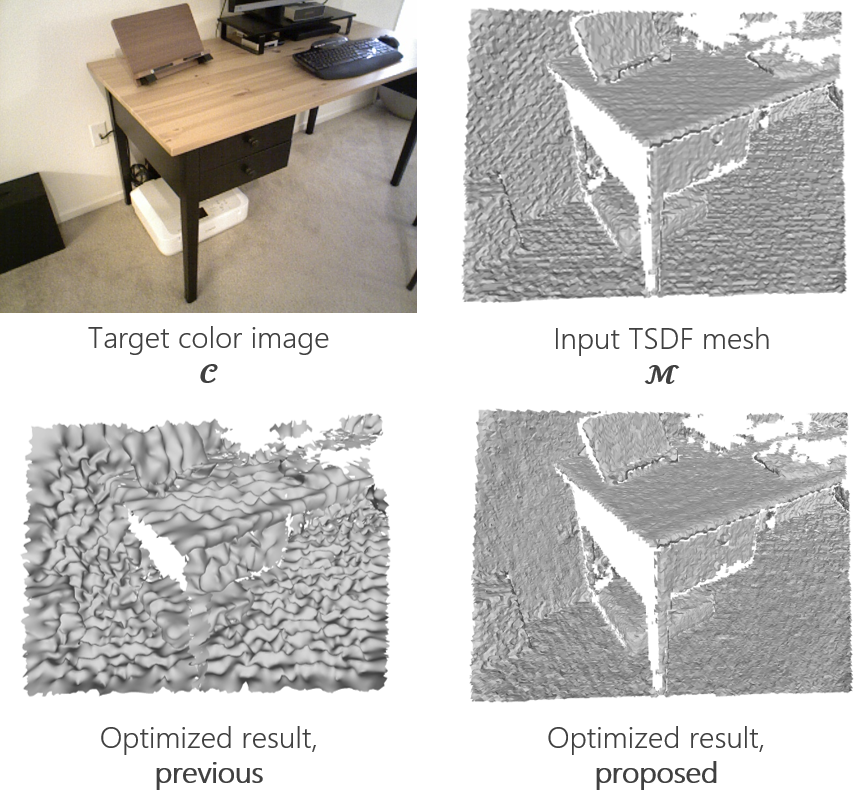
\includegraphics[width=\columnwidth]{figures/4_result_comparison_with_previous_method_simple.png}
    \caption{Equal-iteration comparison of result using previous method\cite{ravi2020accelerating} and our method. 
    % For target silhouette, we generated it from input mesh by render mesh with silhouette renderer, and it is enough to use since silhouette image itself does not hold any depth information other than boundary information of target mesh. \textbf{Previous} result fails to converge to perceptive geometric shape hidden in target images, whereas \textbf{Proposed} result successfully reduces noise. Note that \textbf{Proposed} method only observes $\mathbf{\mathcal{C}}$ in order to infer noise-free geometry, whereas Previous method requires both $\mathbf{\mathcal{C}}$ and $\mathbf{S}$.
    }
    \label{fig:comparison_with_previous_method}
\end{figure}

We compare our method with standard differentiable rendering approach used in differentiable renderer\cite{liu2019soft}. 
We slightly modified its workflow in order to evaluate performance under identical conditions (please refer \ref{fig:difference_simple_mesh_and_tsdf_mesh} for details). 
Specifically, we limit amount of target view to 1, as it is impossible to synthetically generate clean target using existing SLAM sequences. 
For silhouette image, we used silhouette of input TSDF mesh as silhouette itself does not take into account detailed depth information as they represent boundary of mesh \PJ{TODO: to footnote}(Hence, previous methods required silhouette images from different camera extrinsic in order to optimize the shape of input mesh). 
We follow losses and its weights as suggested in previous method\cite{ravi2020accelerating}, which is defined as: 
\begin{multline*}
    \mathcal{L}_{prev}=w_{sil}\cdot L_{sil}+w_{rgb}\cdot L_{rgb}+w_{edge}\cdot L_{edge}+ \\ 
    w_{normal}\cdot L_{normal}+w_{laplacian}\cdot L_{laplacian}, 
\end{multline*}
where $L_{sil}$, $L_{rgb}$ is silhouette, and color difference between input and target, respectively. 
$L_{edge}$, $L_{normal}$, and $L_{laplacian}$ stands for mesh edge length consistency, mesh normal orientation consistency, and mesh Laplacian loss, respectively. 
Note that mesh losses $L_{edge}$, $L_{normal}$, $L_{laplacian}$ is developed from traditional geometry processing field, thus they do not reflect geometric features that are shown in target images. 
For brevity, we skip detailed equations for each loss. 
We used $w_{sil}=1.0$, $w_{rgb}=1.0$, $w_{edge}=1.0$, $w_{normal}=0.01$, $w_{laplacian}=1.0$ as authors suggested.
(Fig. \ref{fig:comparison_with_previous_method}) shows optimized mesh with loss from previous work. 
For target silhouette, we generated it from input mesh, and we empirically found that it is enough to alternate Ground Truth silhouette image. \textbf{Previous} result fails to converge to perceptive geometric shape hidden in target images, whereas \textbf{Proposed} result successfully reduces noise. Note that \textbf{Proposed} method only observes $\mathbf{\mathcal{C}}$ in order to infer noise-free geometry, whereas Previous method requires both $\mathbf{\mathcal{C}}$ and $\mathbf{S}$.
% Resulting mesh preserves its silhouette information, as they provided silhouette loss to prevent vertices to evolve out of its silhouettes. 
% In contrast, vertices within silhouette images are evolved without any shape constraints supervised by target images. 
% Those vertices are guided to satisfy input mesh’s internal properties, as mesh losses does not consider geometric clues in target images. 
% This results in optimized mesh failed to optimize, while only preserving boundary.

\subsection{Limitations \& Future Directions}

We summarize future directions of our method, including failure case and promising extension of proposed method.
\paragraph{Adding Robust Positional Constraint Loss}
Although our method can drastically reduce mesh noise, we found that optimized mesh is not maintaining topologically correct structure. 
Specifically, we observed self-intersections between neighboring faces. 
This problem can be naturally arisen since we did not consider relationship between neighboring vertices in our final loss. 
Therefore, though vertices are evolved to have reduced noise, their evolving direction is totally random, lead to occur self-intersections between neighboring faces by corresponding (incorrectly evolved) neighboring vertices. 
We illustrated this failure case in (Fig. \ref{fig:self_intersection}).


\begin{figure}
    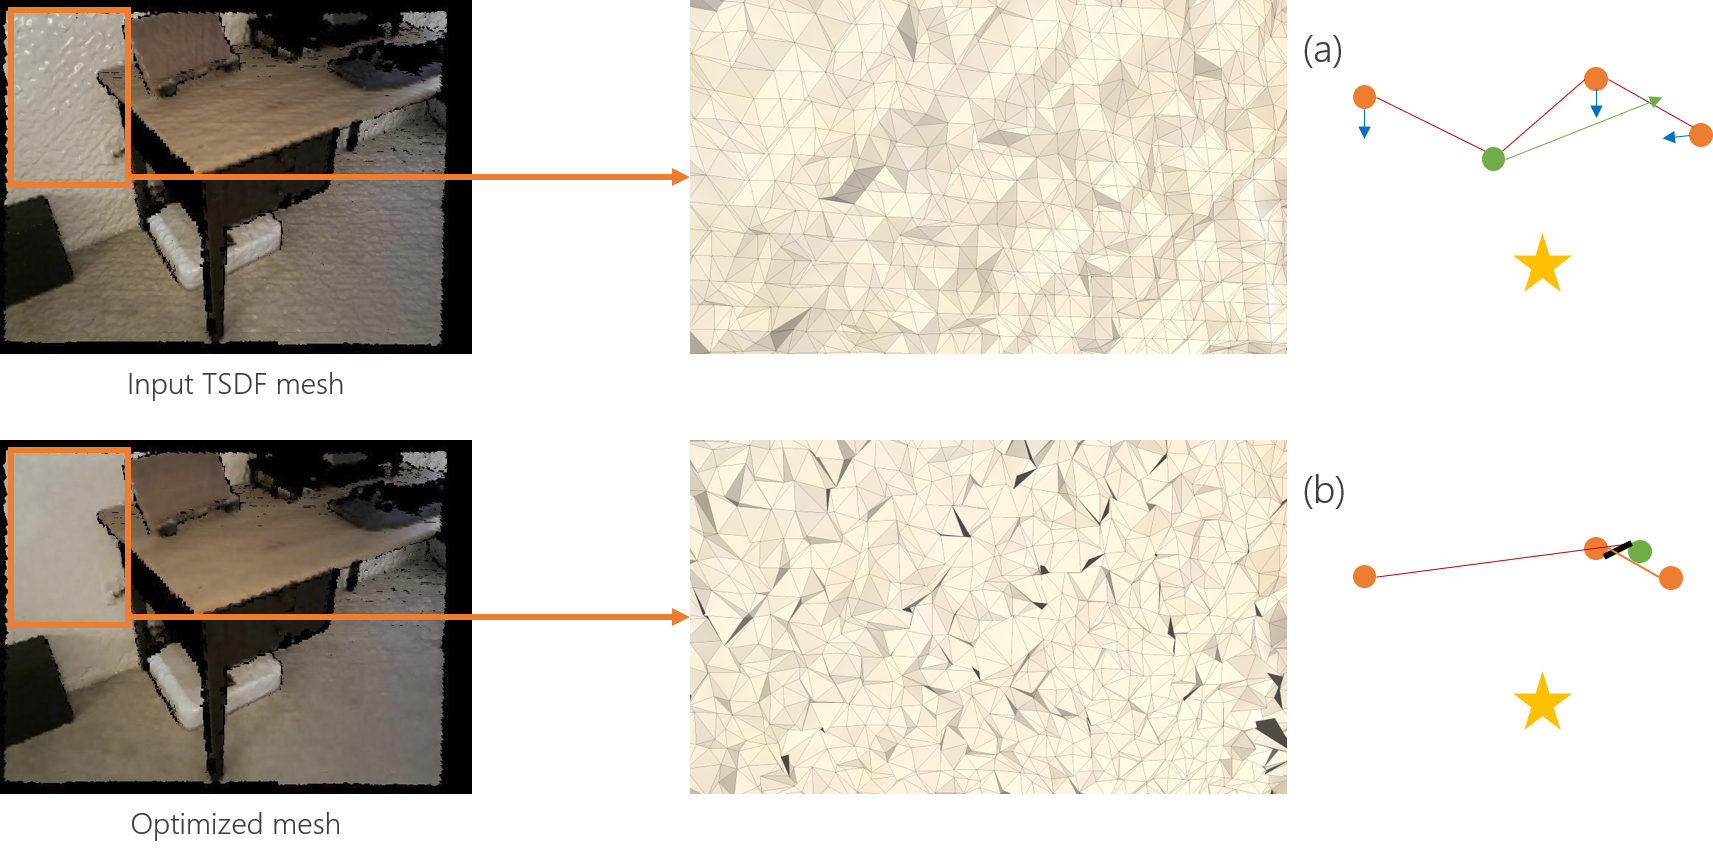
\includegraphics[width=\columnwidth]{figures/4_future_work_self_intersection.png}
    \caption{An example of self-intersection artifact. We zoomed up each geometry corresponds to image inset. 
    \textbf{Black artifacts} are observed in zoomed view in optimized mesh. We found that those are self-intersection between neighboring faces, since our positional constraint $L_{pos}$ does not consider distances between neighboring vertices. 
    This phenomenon is illustrated at the rightmost images of each zoomed view. 
    (a) For each iteration, vertices are optimized while only considering flatness of surfaces, not for topological correctness of geometry. 
    Star, circle, and arrow indicates light position, vertices, and gradient (evolving direction after current optimization step), respectively. 
    Here, \textbf{\textcolor{ForestGreen}{Green vertex}} is optimized to \textbf{\textcolor{ForestGreen}{Green arrow}} direction so that it occludes another face. 
    (b) Consequently, there exists a self-intersection between neighboring faces (\textbf{Black line}) although the entire mesh noise is reduced, resulting self-occluded artifact.}
    \label{fig:self_intersection}
\end{figure}

\paragraph{Edge Fitting}
Although our method is able to minimize noisy vertices by treating $G_\mathcal{C}$ as noise-free geometric clue, however it failed to clean out noisy vertices around geometric edges. 
We found that there is gradient magnitude difference between two images, as on edges $G_{lw}$ tends to have large deviation since it is the place where geometric normal hugely differs. 
Our current $L_2$ loss of gradients cannot reflect this case, as they are evaluated pixel-by-pixel. 
% We visualized this case in (Fig. \ref{fig:edge_fitting}). 
Weighting color gradients by using gradients from depth, say $G_\mathcal{D}$, or developing an erosion kernel for $G_\mathcal{C}$ to reliably cover $G_{lw}$ seems worth trying.

% \begin{figure}
%     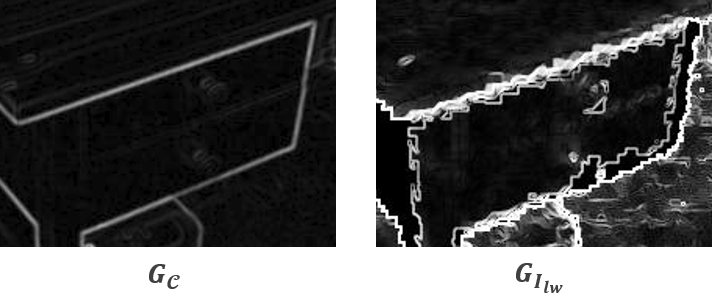
\includegraphics[width=\columnwidth]{figures/4_future_edge_fitting.png}
%     \caption{Inset of each gradient. $G_{lw}$ is corrupted since geometric normal deviates around edge.}
%     \label{fig:edge_fitting}
% \end{figure}
\section{Conclusion}
In this report, we proposed a method that optimizes input TSDF mesh generated from single RGB-D pair, by exploiting noise-free geometric clues hidden in color image. 
Our method differs from most of previous methods as they required to optimize shape from multiple takes of target scene, which is hard to directly apply to SLAM dataset. 
We show that our method outperforms previous differentiable rendering setup. 
Future work on improving robustness in terms of optimizing edgy geometries, preventing topological correctness of input mesh would be beneficial to solve problem that is defined as ill-posed in SLAM.

\bibliographystyle{ACM-Reference-Format}
\bibliography{mc_correction_dr}

\end{document}
